%%%%%%%%%%%%%%%%%%%%%%%%%%%%%%%%%%%%%%%%%%%%%%%%%%%%%%%%%%%%%%%%%%%%%%%%%%%%%%%%
% Template for USENIX papers.
%
% History:
%
% - TEMPLATE for Usenix papers, specifically to meet requirements of
%   USENIX '05. originally a template for producing IEEE-format
%   articles using LaTeX. written by Matthew Ward, CS Department,
%   Worcester Polytechnic Institute. adapted by David Beazley for his
%   excellent SWIG paper in Proceedings, Tcl 96. turned into a
%   smartass generic template by De Clarke, with thanks to both the
%   above pioneers. Use at your own risk. Complaints to /dev/null.
%   Make it two column with no page numbering, default is 10 point.
%
% - Munged by Fred Douglis <douglis@research.att.com> 10/97 to
%   separate the .sty file from the LaTeX source template, so that
%   people can more easily include the .sty file into an existing
%   document. Also changed to more closely follow the style guidelines
%   as represented by the Word sample file.
%
% - Note that since 2010, USENIX does not require endnotes. If you
%   want foot of page notes, don't include the endnotes package in the
%   usepackage command, below.
% - This version uses the latex2e styles, not the very ancient 2.09
%   stuff.
%
% - Updated July 2018: Text block size changed from 6.5" to 7"
%
% - Updated Dec 2018 for ATC'19:
%
%   * Revised text to pass HotCRP's auto-formatting check, with
%     hotcrp.settings.submission_form.body_font_size=10pt, and
%     hotcrp.settings.submission_form.line_height=12pt
%
%   * Switched from \endnote-s to \footnote-s to match Usenix's policy.
%
%   * \section* => \begin{abstract} ... \end{abstract}
%
%   * Make template self-contained in terms of bibtex entires, to allow
%     this file to be compiled. (And changing refs style to 'plain'.)
%
%   * Make template self-contained in terms of figures, to
%     allow this file to be compiled. 
%
%   * Added packages for hyperref, embedding fonts, and improving
%     appearance.
%   
%   * Removed outdated text.
%
%%%%%%%%%%%%%%%%%%%%%%%%%%%%%%%%%%%%%%%%%%%%%%%%%%%%%%%%%%%%%%%%%%%%%%%%%%%%%%%%

\documentclass[letterpaper,twocolumn,10pt]{article}
\usepackage{usenix2019_v3}

% to be able to draw some self-contained figs
\usepackage{tikz}
\usepackage{amsmath}

% inlined bib file
\usepackage{filecontents}

%-------------------------------------------------------------------------------
\begin{document}
%-------------------------------------------------------------------------------

%don't want date printed
\date{}

% make title bold and 14 pt font (Latex default is non-bold, 16 pt)
\title{\Large \bf Non-Fungible Tokens: Project Proposal}

%for single author (just remove % characters)
\author{
{\rm Eason \ Wang}\\
University of California, Berkeley
\and
{\rm Yao Shao}\\
University of California, Berkeley
\and
{\rm Chang Zhou}\\
University of California, Berkeley
\and
{\rm Jiaye Wang}\\
University of California, Berkeley
% copy the following lines to add more authors
% \and
% {\rm Name}\\
%Name Institution
} % end author

\maketitle

%-------------------------------------------------------------------------------
\section{Introduction}
%-------------------------------------------------------------------------------
Non-Fungible Tokens(NFT) as one-of-a-kind digital assets, nowadays, are crazily chased by the Capital and Collectors. It is endowed with a great value by its relative rarity and unique launching mechanism. Hence, understanding the factors that influence NFTs’ price is considerably important. In this project proposal, we presented our plan on extracting key NFT features that influence NFT’s price, and implementing those features using generative adversarial network (GAN). Firstly, we are going to gather NFT’s price data on different NFT trading platforms, such as Opensea. We are going to do data prepossessing and visualization to determine the machine learning model we want to use to extract useful features. Then, we are going to feed those data into various machine learning models to find out which features contribute to the NFT’s price more. After we figure out the features, we are going to select NFTs that include those features and feed them into the generative adversarial network. Lastly, we plan to upload our newly generated NFTs to the NFT’s trading network, and wait for the market response.



% \begin{figure*}[tp]
% 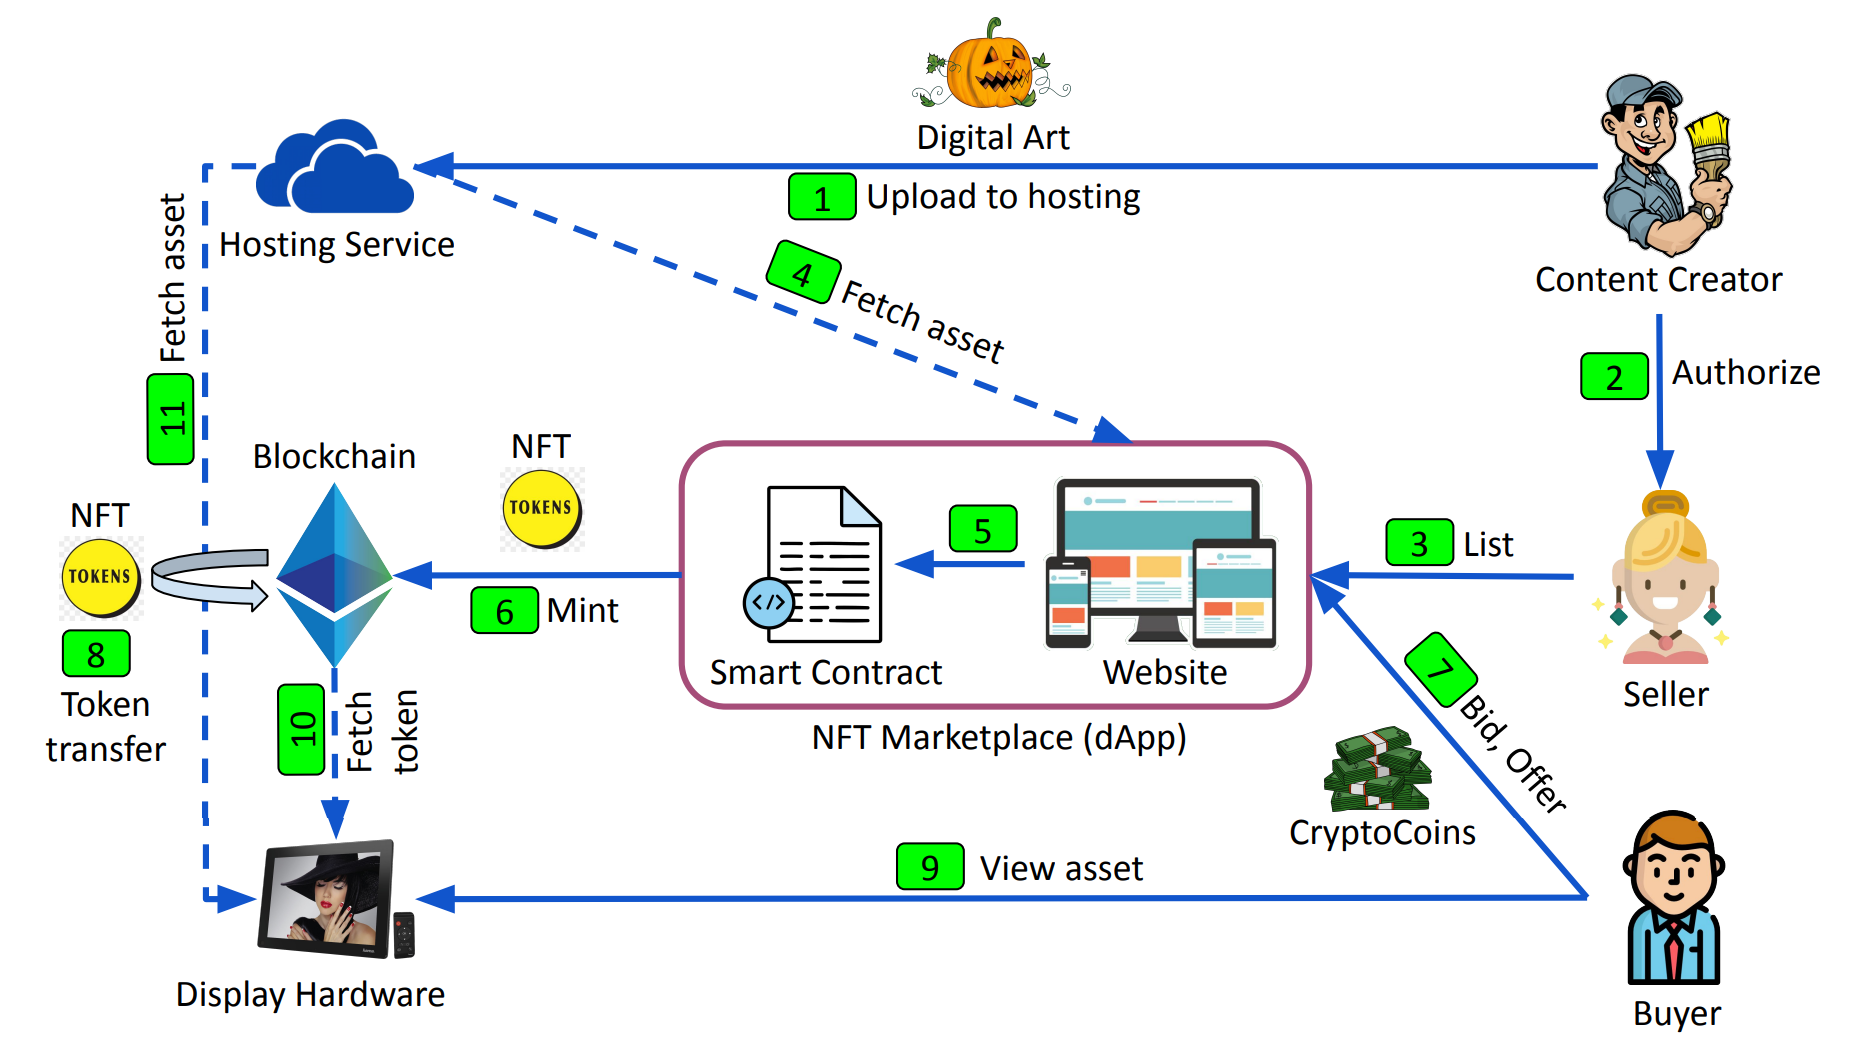
\includegraphics[width=1\textwidth]{Figure/Network Flow.jpg}
% \caption{\label{fig:Network}Non-Fungible Dealing Network Flow}
% \end{figure*}


%-------------------------------------------------------------------------------
\section{Design}
%-------------------------------------------------------------------------------
Our final design will be divided into three parts: exploring and visualizing reliable and appropriate NFTs datasets, building and fitting machine learning models to predict the price of NFTs, and using generative adversarial networks (GANs) to produce some NFTs arts that mimic popular visual elements in existing NFTs. We will discuss each of the three parts in detail in the following subsections. 

\begin{figure}[htbp] \centering 
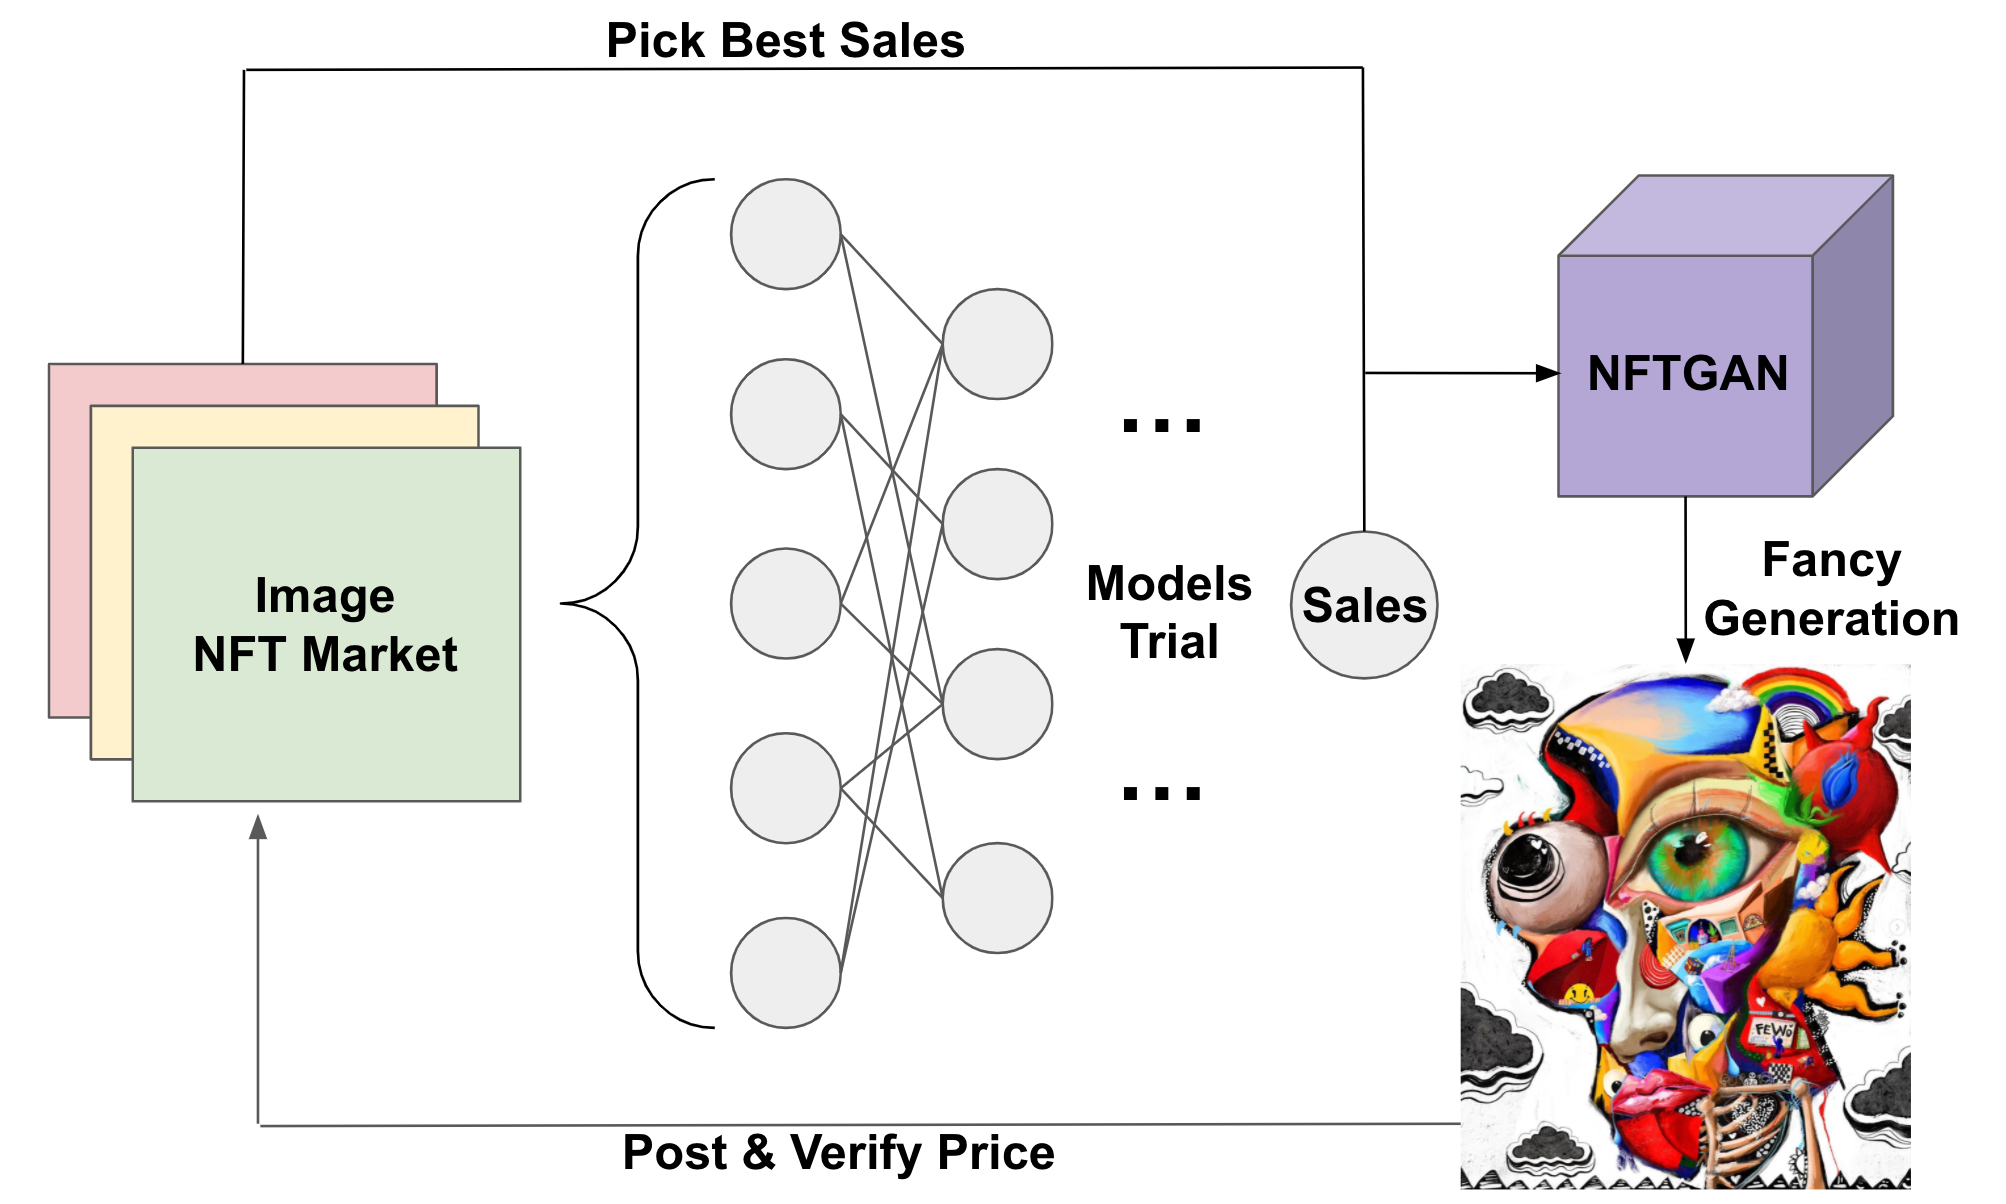
\includegraphics[width=9cm]{Figure/Project Design Flow.jpg} 
\caption{Project Design Flow} 
\label{fig:graph} 
\end{figure} 

\subsection{NFTs Datasets Exploration and Visualization}
After assessing the column features, granularity, completeness, and temporality of different NFTs datasets, we decided to use the Non-Fungible Tokens Dataset created by Matthieu Nadini~\cite{nadini2021mapping}. This dataset contains 6.1 million trades of 4.7 million NFTs between June 23, 2017, and April 27, 2021, in 160 cryptocurrencies, primarily obtained from Ethereum and WAX blockchains~\cite{nadini2021mapping}. This dataset contains in total 24 columns including some crucial information like NFTs name, NFTs collection, NFTs category, NFTs transaction date and time, market, cryptocurrency, image URL, and price. To better understand the Non-Fungible Tokens Dataset created by Matthieu Nadini~\cite{nadini2021mapping}, we will generate some visualizations of this dataset including price distribution of NFTs by category and by time, daily NFTs number of transactions and transaction volumes by category and by cryptocurrency, etc.

\subsection{Machine Learning Models for NFTs Price Prediction}
According to Matthieu’s investigation of the predictability of NFT sales using linear regression, he found that sale history and visual features are the two most important predictors for price~\cite{nadini2021mapping}. We plan to do more explorations using different machine learning models rather than linear regression, for example, decision trees, random forests, RNNs, and DNNs. The output of our machine learning models will be simply the predicted price, and the input to our machine learning models will be features extracted and preprocessed from the Non-Fungible Tokens Dataset like past sales, visual features, cryptocurrency, category, etc. We planned to firstly, use these models to find the most important features for NFTs price prediction, and secondly, compares the performance of these models in making price predictions. 

\subsection{NFTs Generation Using GANs}
Generative adversarial network (GAN) is a type of machine learning framework that consists of two neural network-based models known as generators and discriminators, designed by Ian Goodfellow and his colleagues in June 2014~\cite{goodfellow2014}. GAN has been used widely in generating image content; it has a state-of-art performance. Therefore, we planned to select some NFTs trades with top price from the Non-Fungible Tokens Dataset. We will later use the pre-trained GAN to do some fine tuning and newly generate some NFTs visuals, releasing them into the NFTs market. Then, we will utilize our part1 price predictor to give a forecasting price and further compare our predicting price with the real market response price, finally verifying the correctness and value of our project.


%-------------------------------------------------------------------------------
\section{Implementation}
%-------------------------------------------------------------------------------

\subsection{Newly Designed NFT Sale Predictor}
As Matthieu mentioned in his paper - Mapping the NFT revolution: market trends, trade networks, and visual features\cite{nadini2021mapping}, they investigated the predictability of NFT sales and locked on several features as useful factors influencing the price of NFTs. But, the predicting model they choose is relatively simple(Linear Regression). Therefore, We are planning to add to this part, make a trial to use and compare different machine learning or deep learning models.Besides, if possible, we will try to dig out more conducive features that may contribute to our final prediction. Finally, we are expecting to implement a better sales predictor with newly designed forecasting models and new features.

\subsection{NFTGAN-NFT Arts Creation Booster}
Based on the research of part1, we could proactively pick out a group of NFT artworks(Image) with relatively beautiful saling properties. Taking these artworks as the input, we are going to utilize current popular Generative adversarial Networks(GAN) to generate some brand new artworks, aiming at boosting the creation process for artists, catching trending favor of the public and doing some agile creation. For part2, we mainly consider the visual features of the input artworks and expect doing so would help the artists and salers to make more profit. Here, I have to point out that regarding the lack of history data of the same type of experiment, we plan to keep this part as a long-term open-ended question. We will post our newly generated artworks to the NFT market to collect the real sales data as the market response(need more time, may continue after the end of this class) and fine tune our generation models later.


% \begin{figure}[htbp] \centering 
% 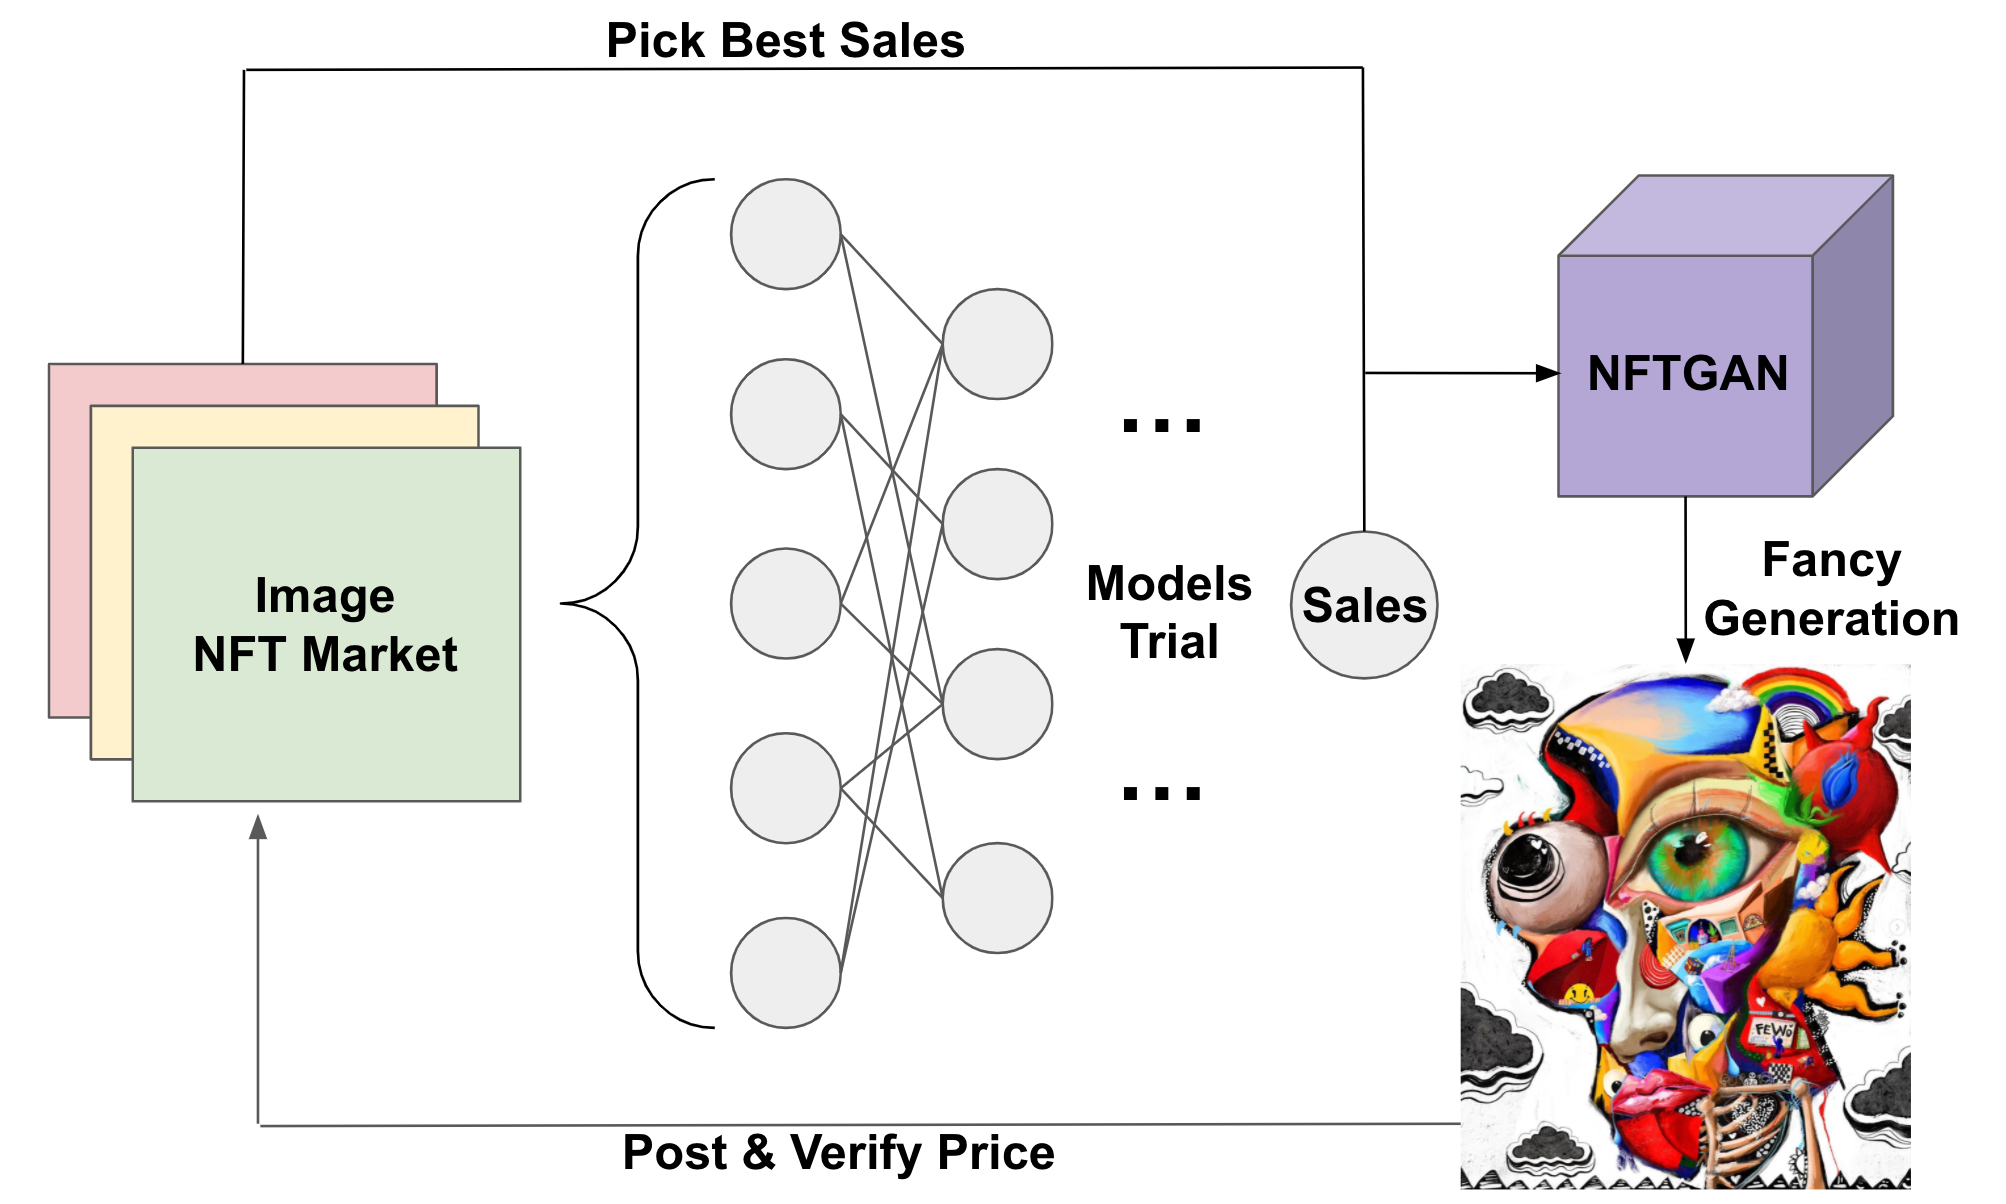
\includegraphics[width=9cm]{Figure/Project Design Flow.jpg} 
% \caption{Project Design Flow} 
% \label{fig:graph} 
% \end{figure} 

% \begin{figure}[htbp]
% 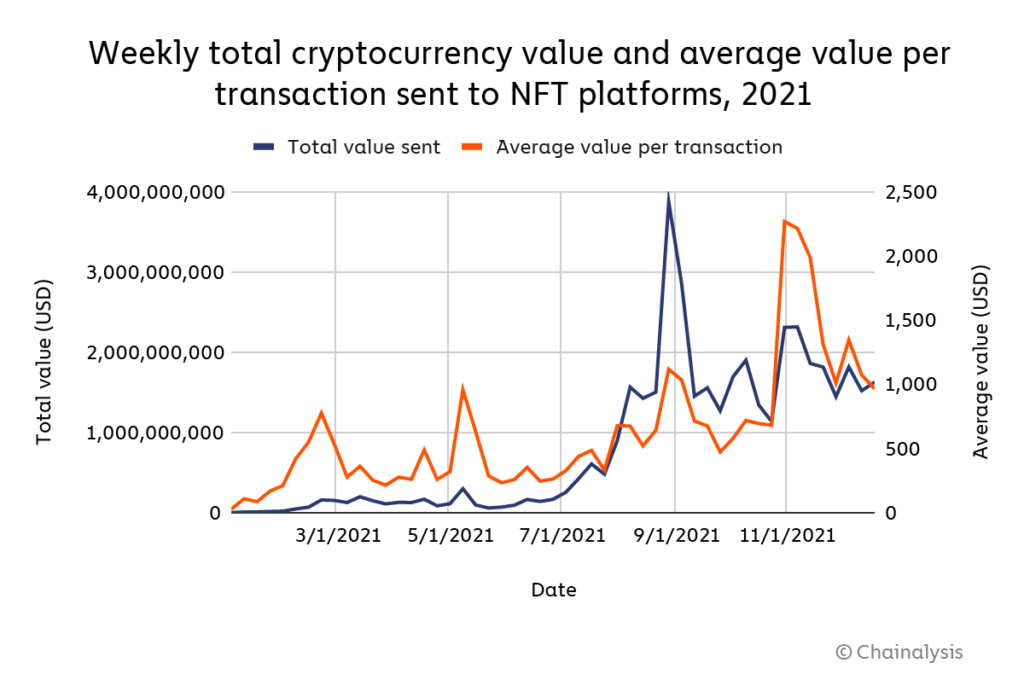
\includegraphics[width=0.5\textwidth]{Figure/The weekly total cryptocurrency value.png}
% \caption{The weekly total cryptocurrency value and average value per transaction sent to NFT platforms in 2021.~\cite{tumblr_team_2022}}
% \label{fig:week}
% \end{figure}


%-------------------------------------------------------------------------------
\section{Evaluation}
%-------------------------------------------------------------------------------
After careful design and implementation, we will now focus on how to evaluate our approach. Since our project can be divided into three parts: Analysis and visualization of NFT Markets, predicting prices of NFTs, and generate new NFTs that produce higher profit. Each of these parts has a different objective so requires diverse evaluation methods. 

For market analysis, we will use different visualization methods to comprehensively analyze NFT market trading information and extract unique user behavior features. The main evaluation criteria are comprehensiveness, depth and innovation of the analysis.

For NFT generations, we aims to produce brand new images that may have a higher selling price. Since we will apply GAN, possible experiments could be training and testing the model on the dataset with millions of NFTs and transactions. To evaluate the performance of the model, we will compare the predicted prices of newly generated NFTs with existed NFTs. We may also publish some of the created NFTs in open market and analysis their primary and second sale prices if possible.

For price prediction, the objective is to design a ML based algorithm that can predict NFT price as accurate as possible. The corresponding experiments and evaluation metrics are discussed in the following sections.

\subsection{Experiments Design}
We will evaluate the performance of our approach by testing on open datasets with millions of past and recent NFT transactions in a long time window. We will compare our model with many other machine learning models, such as linear regression, SVM, AdaBoost, convolutional neural networks (CNNs) and recurrent neural networks (RNNs), etc. The performance and predictive power of our method on different types of data sources and data types will also be a direction of the evaluation. 

\subsection{Evaluation Metrics}
Since price prediction can be viewed as a regression task, we will apply three kinds of metrics that is widely used in evaluating regression models.

\textbf{R Square/Adjusted R Square}: R Square measures how much variability in dependent variable can be explained by the model. It is the square of the Correlation Coefficient(R) and that is why it is called R Square.
$$R^{2}=1-\frac{S S_{R e g r e s s i o n}}{S S_{\text {Total }}}=1-\frac{\sum_{i}\left(y_{i}-\hat{y}_{i}\right)^{2}}{\sum_{i}\left(y_{i}-\bar{y}\right)^{2}}$$
R Square is calculated by the sum of squared of prediction error divided by the total sum of the square which replaces the calculated prediction with mean. R Square value is between 0 to 1 and a bigger value indicates a better fit between prediction and actual value.

\textbf{Mean Square Error(MSE)}: While R Square is a relative measure of how well the model fits dependent variables, Mean Square Error is an absolute measure of the goodness for the fit.
$$M S E=\frac{1}{N} \sum_{i=1}^{N}\left(y_{i}-\hat{y}_{i}\right)^{2}$$
MSE is calculated by the sum of square of prediction error which is real output minus predicted output and then divide by the number of data points. It gives us an absolute number on how much our predicted results deviate from the actual number.

\textbf{Mean Absolute Error(MAE)}: Mean Absolute Error(MAE) is similar to Mean Square Error(MSE). However, instead of the sum of square of error in MSE, MAE is taking the sum of the absolute value of error.
$$M A E=\frac{1}{N} \sum_{i=1}^{N}\left|y_{i}-\hat{y}_{i}\right|$$
Compare to MSE, MAE is a more direct representation of sum of error terms. MSE gives larger penalization to big prediction error by square it while MAE treats all errors the same.

%-------------------------------------------------------------------------------
\section{Discussion}
%-------------------------------------------------------------------------------

In the last step of our project, we only upload our newly generated NFTs to the market. However, according to our lecture, the price of NFTs needs some time to stabilize. Hence, we will need to monitor our new NFT price in order to prove our extracted feature is actually relevant to NFT’s price. Another possible point is the background information of NFTs. Most popular NFTs usually have something to support them. For example, many celebrities have made some NFTs and sell those NFTs for an extremely high price. However, we are not able to include those parts in our project. Hence, we are not able to control all variables in our experiment and may cause our result to be insufficient. Our team is not sure about the result of our research since it will take time to prove the result.

%-------------------------------------------------------------------------------
\section{Milestones \& Task Assignment}
%-------------------------------------------------------------------------------
The plan of task division is as follows:

Part1: Dataset Visualization: Jiaye Wang \& Chang Zhou \& Eason Wang \& Yao Shao

Part2: Prediction model design and implementation: Jiaye Wang \& Chang Zhou

Part3: NFTGAN design and implementation: Eason Wang \& Yao Shao

% Post newly generated NFTs to the market: Jiaye Wang 

\begin{figure}[htbp] \centering 
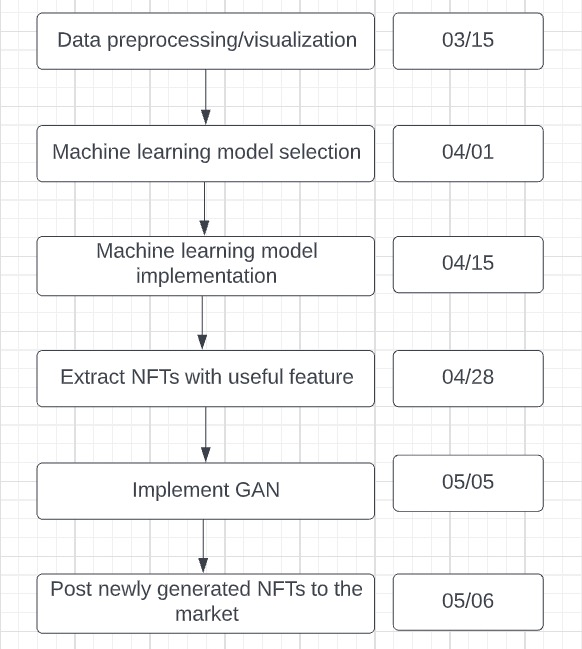
\includegraphics[width=8cm]{Figure/Timeline.jpeg} 
\caption{Milestone and Project Timeline} 
\label{fig:graph} 
\end{figure} 
%-------------------------------------------------------------------------------
\bibliographystyle{plain}
\bibliography{Cite}

%%%%%%%%%%%%%%%%%%%%%%%%%%%%%%%%%%%%%%%%%%%%%%%%%%%%%%%%%%%%%%%%%%%%%%%%%%%%%%%%
\end{document}
%%%%%%%%%%%%%%%%%%%%%%%%%%%%%%%%%%%%%%%%%%%%%%%%%%%%%%%%%%%%%%%%%%%%%%%%%%%%%%%%

%%  LocalWords:  endnotes includegraphics fread ptr nobj noindent
%%  LocalWords:  pdflatex acks